\chapter{矩阵与线性映射}
\begin{center}
	\textcolor[RGB]{255, 0, 0}{\faHeart}所以生命啊,它苦涩如歌.\textcolor[RGB]{255, 0, 0}{\faHeart}
\end{center}
\rightline{——《我用什么把你留住》}
\vspace{-5pt}
\begin{center}
	\pgfornament[width=0.36\linewidth,color=lsp]{88}
\end{center}

\section{线性方程组与矩阵}

\subsection{线性方程组与平面上的线性变换}

回顾初中所学的一些内容,我们了解到了二元一次方程组,它们形如:
$$\left\{\begin{matrix} 
	a_1x+b_1y=c_1 \\  
	a_2x+b_2y=c_2
  \end{matrix}\right. $$
这就是线性方程组的一种,通常可用于平面上的线性变换,下面一种情况就是平面上的线性变换:
\begin{figure}[htbp]
	\centering
	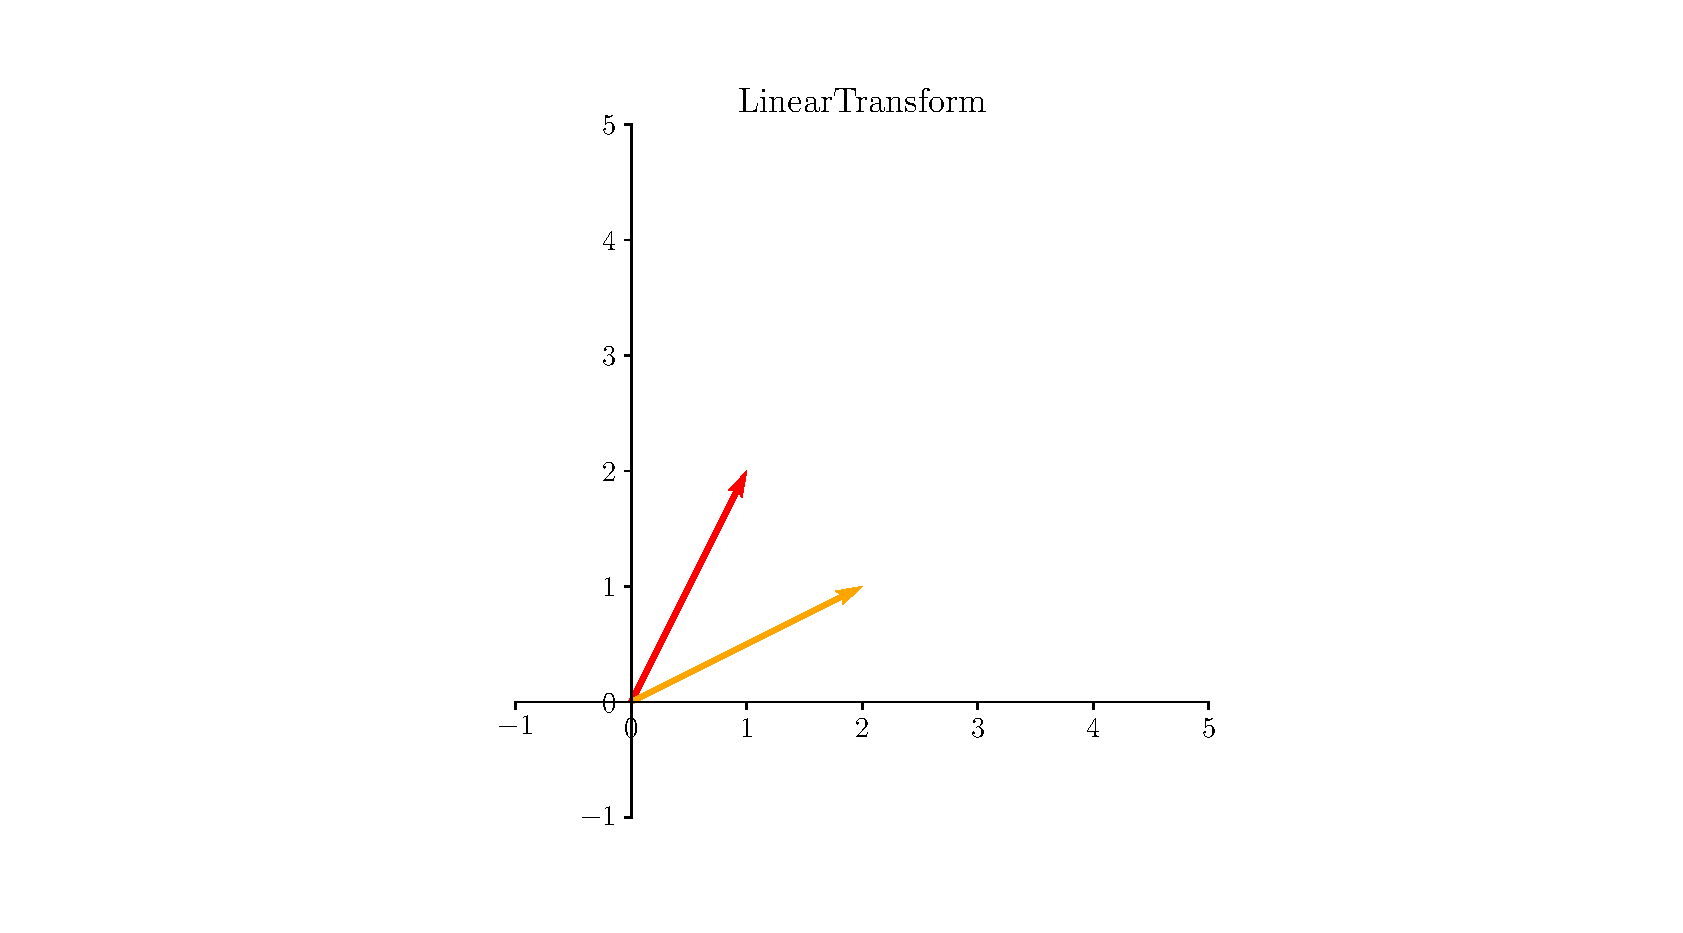
\includegraphics[width=0.7\linewidth]{figure/eps/LinearTransform.eps}
	\caption{线性变换}
	\label{fig:LinearTransform}
\end{figure}

我们平常所使用的坐标系是直角坐标系,表示向量使用标准基$\left\{ (1,0),(0,1) \right\}$,所谓的线性变换是指如果将坐标系进行一个变化,使得构成这个系的基由原来的$\left\{ (1,0),(0,1) \right\}$变化成$\left\{ (x_1,y_1),(x_2,y_2) \right\}$后所表示的向量在原坐标系中所表示的坐标。如图\ref{fig:LinearTransform}所示,如果我们的基由原来的$\left\{ (1,0),(0,1) \right\}$变化成$\left\{ (1,2),(2,1) \right\}$,那么变换前坐标$(4,5)$的线性组合是$(4,5)=4(1,0)+5(0,1)$,而变化基后的坐标则变为$(14,13)=4(1,2)+5(2,1)$,即空间内的每一点$(x,y)=x(1,0)+y(0,1)$都变化为$(x+2y,2x+y)=x(1,2)+y(2,1)$,设变化后的空间的每一个点在原坐标系的坐标表示为$(x',y')$;表示为线性方程组就是$$\left\{\begin{matrix} 
	1x+2y=x' \\  
	2x+1y=y'
  \end{matrix}\right. $$如果我们把这个式子进一步抽象,可以得到一个矩阵方程$$\begin{pmatrix}  
	1 & 2 \\  
	2 & 1  
  \end{pmatrix} \begin{pmatrix}  
	x \\  
	y  
  \end{pmatrix} =\begin{pmatrix}  
	x' \\  
	y'  
  \end{pmatrix}$$

\begin{example}
	在平面直角坐标系中,向量$a=\overrightarrow{OP_1}=(3,2),b=\overrightarrow{OP_2}=(4,7)$;
	\begin{enumerate}
		\item 求$\triangle OP_1P_2$的面积;
		\item 若将$x$轴的每一个值扩大一倍,求标准基经过变换后的向量集合;
		\item 若将$y$轴的每一个值扩大一倍,求变换后的三角形面积$\triangle OP_1'P_2'$
	\end{enumerate}
\end{example}